\label{packagemaster1}

%Package Listing

\usepackage{tgbonum}
\usepackage[paperwidth=6in,paperheight=9in,inner=0.75in,outer=0.75in,tmargin=1.2in,bmargin=0.8in]{geometry}%paperwidth=6in,paperheight=9in,inner=1.0in,outer=0.5in,tmargin=1.2in,bmargin=0.8in
\usepackage{fancyhdr}
\pagestyle{fancy}
\usepackage{setspace}
\usepackage[T1]{fontenc}
\usepackage{bm}
\usepackage{bibentry}
\usepackage{subcaption}
\usepackage{wrapfig}
\usepackage{amsmath}
\usepackage{mathtools}
\usepackage[inline]{enumitem}
\usepackage{booktabs}
\usepackage[colorlinks, hyperindex]{hyperref}
\usepackage[usenames,dvipsnames,pdftex]{xcolor}
\usepackage{tikz}
\usetikzlibrary{backgrounds,shapes,arrows,positioning,calc,snakes,fit}
\usepgflibrary{decorations.markings}
\usepackage{graphicx} 
\usepackage{todonotes} 
\usepackage[ddmmyyyy,12hr]{datetime}
\renewcommand{\dateseparator}{.}
\usepackage{amssymb}
\usepackage{amsthm}
\usepackage{thmtools}
\usepackage[numbers]{natbib}
\bibliographystyle{plainnat} 
\usepackage{listings}
\usepackage{color}
\usepackage{sectsty}
\usepackage[most]{tcolorbox}
\usepackage{mathrsfs}
\usepackage{caption}
\usepackage{multicol}
\usepackage[margin=10pt, font=footnotesize, labelfont=bf, labelsep=colon]{caption}
\usepackage{breqn}
\catcode`_=12
\catcode`^=12
\usepackage{tensor}
\usepackage{imakeidx}
\usepackage[rule=0.2pt,indentunit=0.75em, initsep=10 pt plus 5 pt minus 3 pt, font=footnotesize, totoc=true]{idxlayout}
\usepackage[titles,subfigure]{tocloft}
\usepackage{minitoc}
\usepackage{etoolbox}
\usepackage{float}
\usepackage[flushmargin, hang]{footmisc}
\usepackage{physics}
\usepackage{slashed}
\usepackage[version=4]{mhchem}
\usepackage{marginnote}
\usepackage[toc,page]{appendix}
\usepackage{microtype}

% Appendix Styling

\renewcommand\appendixpagename{Appendices
%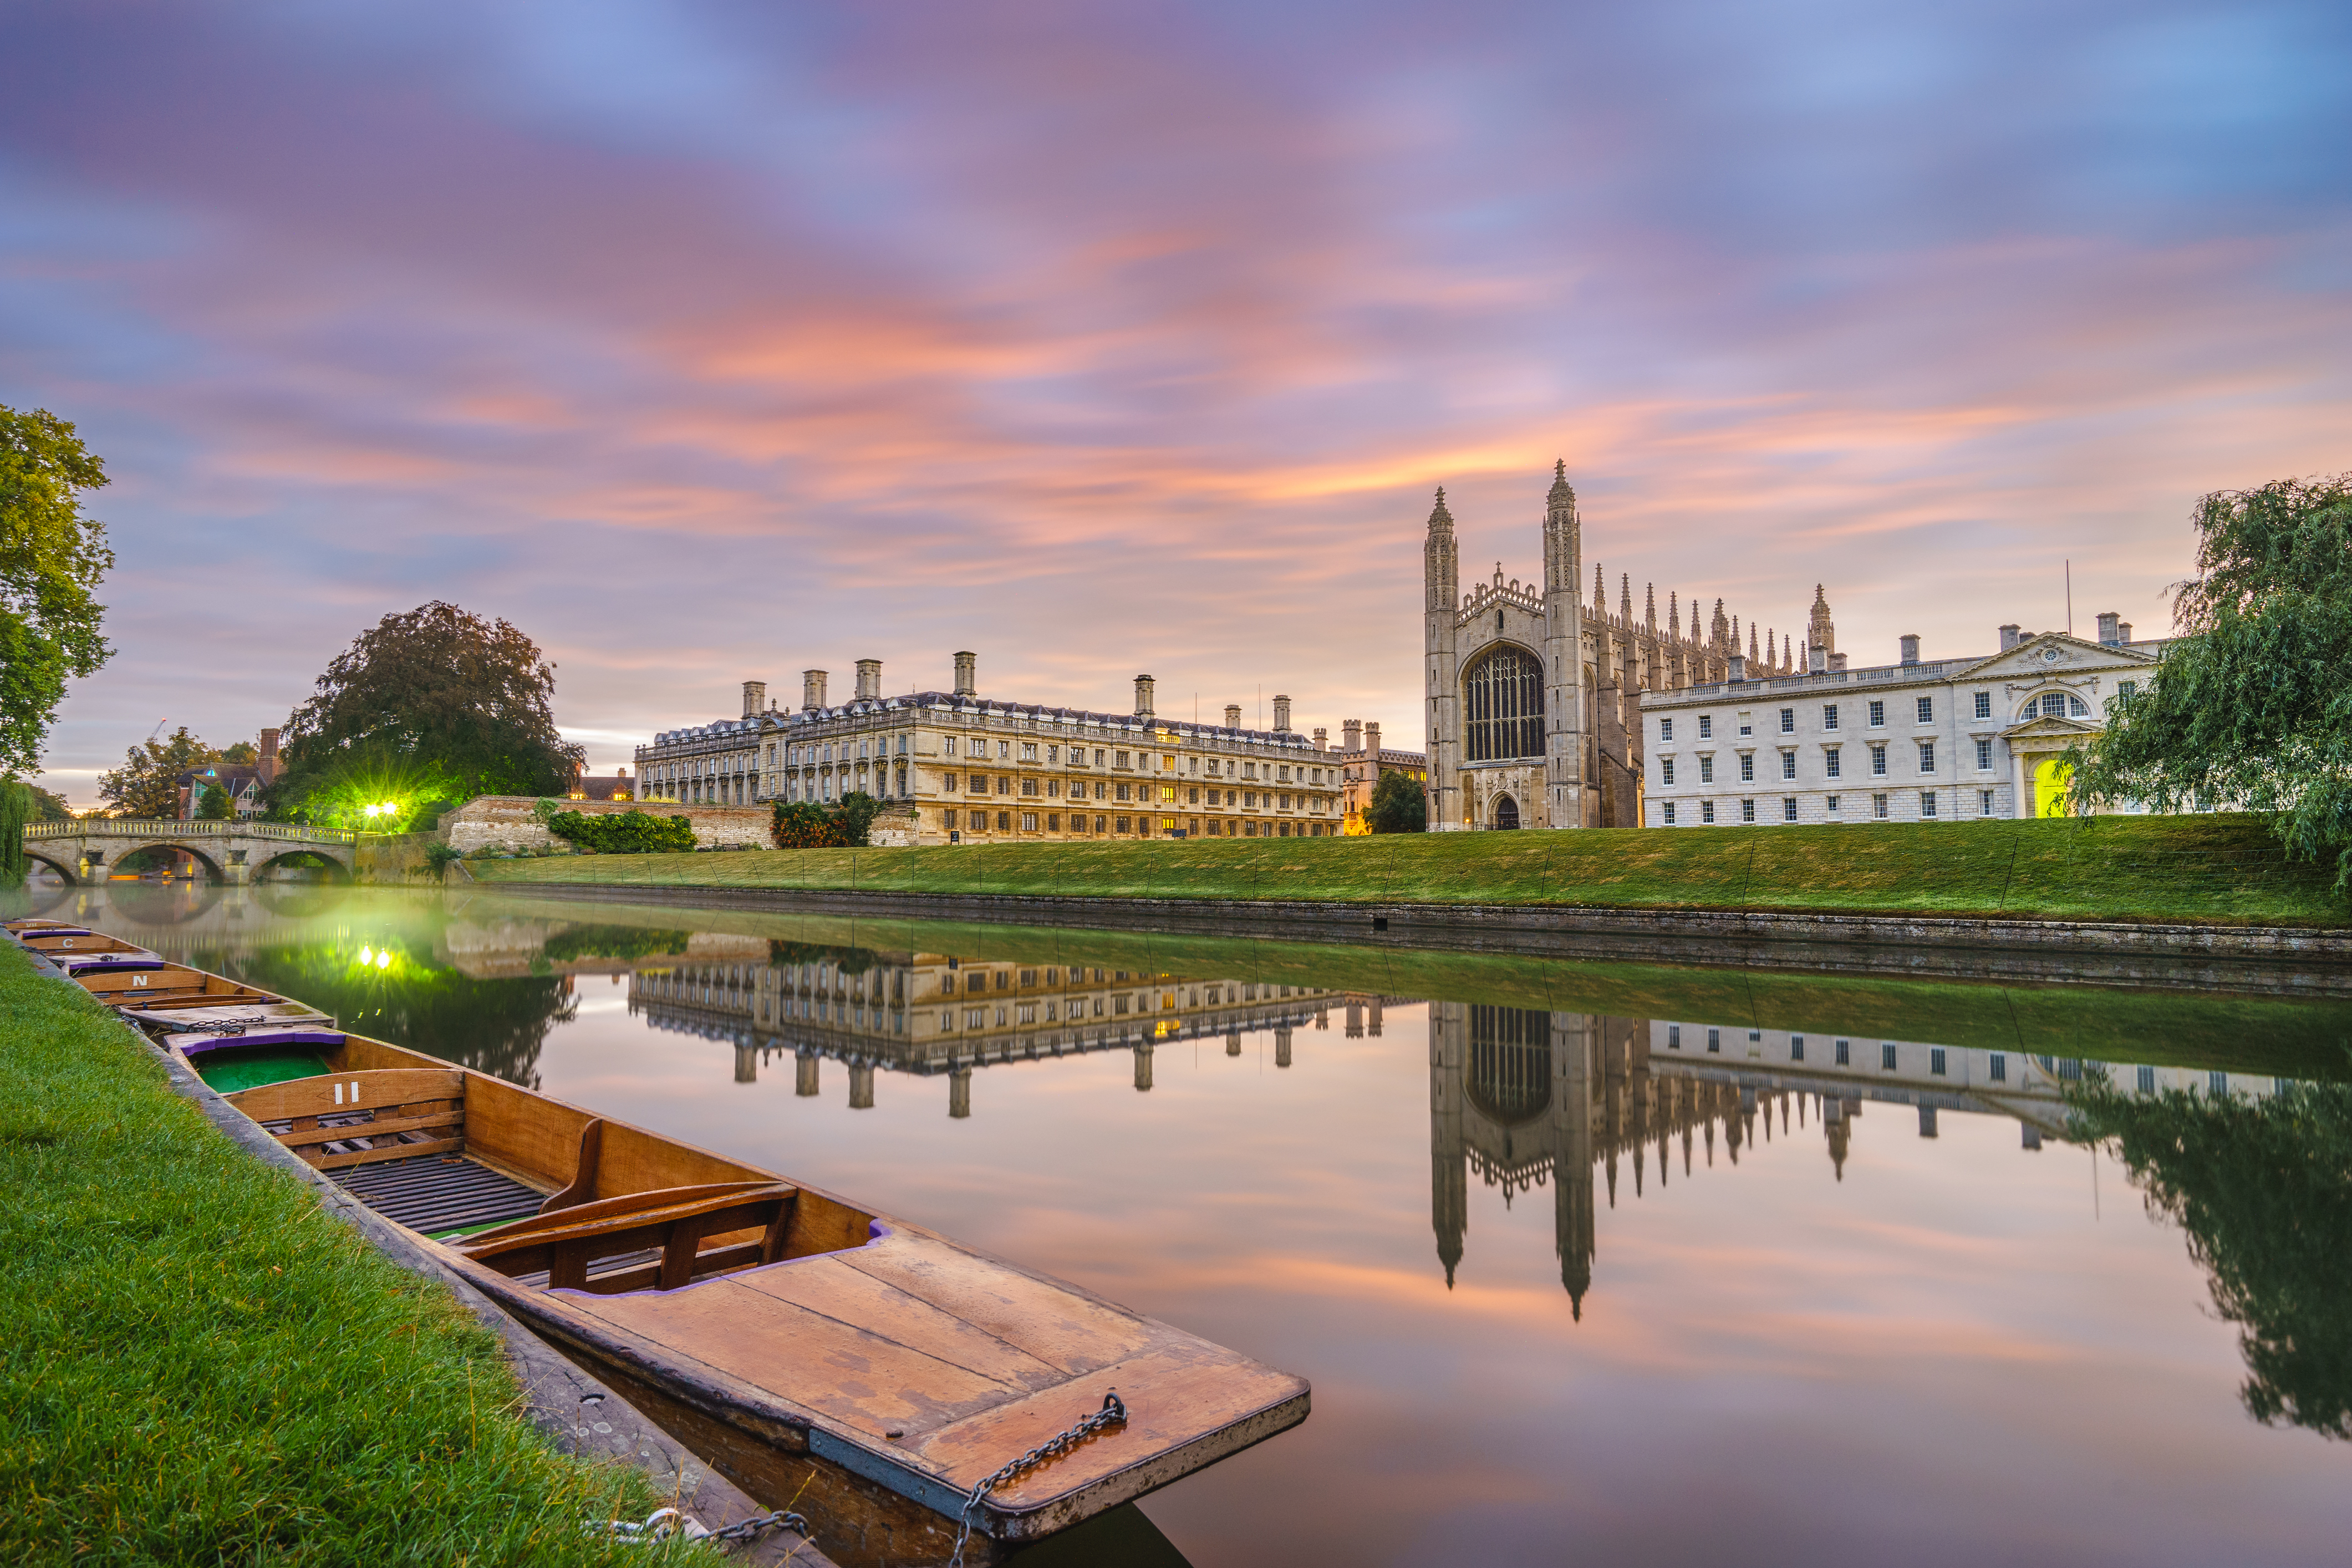
\includegraphics[width=\textwidth]{graphics/cambridge.jpg}
}
\renewcommand\appendixtocname{Appendix}

% Inline equation numbering

\newcommand\inlineeqno{\stepcounter{equation}\ (\theequation)}

% Footnotes

\addtolength{\footnotesep}{1mm}
\setlength{\footnotemargin}{1em}
\numberwithin{footnote}{chapter}
\renewcommand{\thefootnote}{\textbf{\arabic{footnote}}}
\renewcommand\footnoterule{{\hrule height 0.2pt}}

% Caption setup

\captionsetup[table]{position=bottom}

% Chapter styling

\makeatletter
\patchcmd{\@makechapterhead}{\bfseries}{\relax}{}{}% Non-bold \chapter name
\patchcmd{\@makechapterhead}{\bfseries}{\relax}{}{}% Non-bold \chapter title
\makeatother

% ToC styling

\setcounter{tocdepth}{3}
\renewcommand{\cftdot}{.}
\renewcommand{\cftdotsep}{0.5}
\renewcommand{\cftsecdotsep}{2}
\setlength{\cftbeforechapskip}{20pt}
\setlength{\cftbeforesecskip}{3pt plus.2pt}
\setlength{\cftbeforesubsecskip}{2pt}
\cftsetindents{chapter}{0in}{0.4in}
\cftsetindents{section}{0.5in}{0.3in}
\cftsetindents{subsection}{0.85in}{0.4in}
\cftsetindents{subsubsection}{0.95in}{0.4in}
\renewcommand{\cftchapleader}{\hspace{2pt}\small\cftdotfill{\cftdotsep}}
\renewcommand{\cftsecleader}{\hfill}
\renewcommand{\cftsubsecleader}{\hfill}
\renewcommand{\cftsecpagefont}{\small}
\renewcommand{\cftsubsecpagefont}{\small}
\renewcommand\cftchapfont{\normalsize\scshape}
\renewcommand{\cftsecfont}{\small\bfseries}
\renewcommand{\cftsubsecfont}{\small}
\renewcommand{\cftsubsubsecfont}{\footnotesize}
\cftpagenumbersoff{subsection}
\cftpagenumbersoff{subsubsection}
\renewcommand*{\contentsname}{Courses}

% Mini ToC styling

\setcounter{minitocdepth}{3}
\setlength{\mtcindent}{0pt} 
\renewcommand{\mtcfont}{\tiny\rm} 
\renewcommand{\mtcSfont}{\small\rm}
\renewcommand{\mtctitle}{}

%Index setup

\makeindex[title=Index, columns=2, columnseprule=true]
\indexsetup{othercode=\footnotesize}

%\doublespacing (optional)

% Section labelling

\chapterfont{\centering \Huge \textsc}
\sectionfont{\centering \Large \textsc}
\subsectionfont{\large}
\subsubsectionfont{\normalsize}
\renewcommand\thechapter{\arabic{chapter}}
\renewcommand\thesection{\Roman{section}\hspace{-5pt}}
\renewcommand\thesubsection{\arabic{section}.\arabic{subsection}}
\setcounter{secnumdepth}{3} % If you want subsubsections numbered
\renewcommand\thesubsubsection{\arabic{section}.\arabic{subsection}.\arabic{subsubsection}}

% Equation, figure, and table numbering

\numberwithin{equation}{section}
\renewcommand\theequation{\arabic{section}.\arabic{equation}}
\numberwithin{figure}{section}
\renewcommand\thefigure{\arabic{section}.\arabic{figure}}
\numberwithin{table}{section}
\renewcommand\thetable{\arabic{section}.\arabic{table}}

% Theorem definition, numbering, and styling

\newtheoremstyle{mystyle}{\topsep}{\topsep}{\normalfont}{}{\bfseries}{:}{.5em}{}
\theoremstyle{mystyle}
\newtheorem{theorem}{Theorem}
\newtheorem*{example}{Example}
\newtheorem*{definition}{Definition}
\numberwithin{theorem}{section}
\renewcommand\thetheorem{\arabic{section}.\arabic{theorem}}

% Itemize and enumerate styling

\renewcommand{\labelitemi}{\raisebox{0.5ex}{\tiny$\bullet$}}
\renewcommand{\labelenumi}{\raisebox{0.15ex}{\footnotesize\textbf{\arabic{enumi})}}}
\setlist[itemize]{leftmargin=0.4in}
\setlist[enumerate]{leftmargin=0.4in}

% Paragraph, and multicols setup

\setlength{\parindent}{0pt}
\setlength{\columnsep}{1cm}
\setlength{\columnseprule}{0.1pt}

% Document hyperlink setup

\hypersetup{colorlinks=true,linkcolor=black}

% Operator and command definitions

\DeclareMathOperator\artanh{artanh}
%\DeclareMathOperator{\sech}{sech}
\DeclareMathOperator{\sgn}{sgn}
\DeclareMathOperator{\vecspan}{span}
\DeclareMathOperator{\cosec}{cosec}

\renewcommand\vec{\mathbf}
\newcommand{\normord}[1]{\raisebox{0.5pt}{:}\,#1\,\raisebox{0.5pt}{:}}
\newcommand{\dagg}{^{\dagger}}
\newcommand{\pr}{^{\prime}}
\newcommand{\nhat}{\hat{\bm{n}}}
\newcommand{\hamilt}{\mathcal{H}}
\newcommand{\mA}{\mathcal{A}}
\newcommand{\mW}{\mathcal{W}}
\newcommand{\mN}{\mathcal{N}}
\newcommand{\mD}{\mathcal{D}}
\newcommand{\mS}{\mathcal{S}}
\newcommand{\mL}{\mathcal{L}}
\newcommand{\mC}{\mathcal{C}}
\newcommand{\mO}{\mathcal{O}}
\newcommand{\mM}{\mathcal{M}}
\newcommand{\mT}{\mathcal{T}}
\newcommand{\mZ}{\mathcal{Z}}
\newcommand{\mR}{\mathcal{R}}
\newcommand{\II}{\mathbb{I}}
\newcommand{\RR}{\mathbb{R}}
\newcommand{\ZZ}{\mathbb{Z}}
\newcommand{\CC}{\mathbb{C}}
\newcommand{\FF}{\mathbb{F}}
\newcommand{\lie}[1]{\mathcal{L}\left(#1\right)}
\renewcommand{\abs}[1]{\left|#1\right|}
\newcommand{\set}[1]{\left\{#1\right\}}
\newcommand{\SO}[1]{\textrm{SO}\left(#1\right)}
\newcommand{\SU}[1]{\textrm{SU}\left(#1\right)}
\newcommand{\Orth}[1]{\textrm{O}\left(#1\right)}
\newcommand{\Uni}[1]{\textrm{U}\left(#1\right)}
\newcommand{\paraskip}{\vspace{10pt}}
\newcommand*\diff{\mathop{}\!\mathrm{d}}
\newcommand{\del}{\partial}
\newcommand{\TeG}{\mathcal{T}_e(\mathscr{G})}
\newcommand{\TpM}{\mathcal{T}_p(\mathcal{M})}
\newcommand{\TpMs}{\mathcal{T}^{\star}_p(\mathcal{M})}
\newcommand{\etamn}[1]{\eta#1{\mu \nu}}
\newcommand{\upd}[1]{\text{d}#1 \,}
\newcommand{\ud}{\text{d}}
\newcommand{\group}{\mathscr{G}}
\newcommand{\alge}{\mathfrak{g}}
\newcommand{\twobytwo}[4]{\begin{pmatrix}#1&#2 \\ #3&#4 \end{pmatrix}}
\newcommand{\thrbythr}[3]{\begin{pmatrix}#1 \\ #2 \\ #3\end{pmatrix}}
\newcount\colveccount
\newcommand*\colvec[1]{
        \global\colveccount#1
        \begin{pmatrix}
        \colvecnext
}
\def\colvecnext#1{
        #1
        \global\advance\colveccount-1
        \ifnum\colveccount>0
                \\
                \expandafter\colvecnext
        \else
                \end{pmatrix}
        \fi
}

% Colour definitions and code input

\definecolor{codegreen}{rgb}{0,0.6,0}
\definecolor{codegray}{rgb}{0.5,0.5,0.5}
\definecolor{codepurple}{rgb}{0.58,0,0.82}
\definecolor{backcolour}{rgb}{0.95,0.95,0.92}
\definecolor{namecolor}{cmyk}{1,.60,0,.40}
\definecolor{titlepagecolor}{cmyk}{1,.10,0,.10} 

\lstdefinestyle{mystyle}{
  backgroundcolor=\color{backcolour}, commentstyle=\color{codegreen},
  keywordstyle=\color{magenta},
  numberstyle=\tiny\color{codegray},
  stringstyle=\color{codepurple},
  basicstyle=\footnotesize,
  breakatwhitespace=false,
  breaklines=true,
  captionpos=b,
  keepspaces=false,
  numbers=right,
  numbersep=4pt,
  showspaces=false,
  showstringspaces=false,
  showtabs=false,
  tabsize=2
}
\lstset{style=mystyle}

% tcolorbox stylings

\newtcolorbox{chapterbox}[1][]{enhanced,arc=0.1mm,auto outer arc, colback=white!5!white,colframe=red!75!black,leftrule=1pt,rightrule=1pt,toprule=1pt,bottomrule=1pt,left=0mm,right=0mm}

\newtcolorbox{examplebox}[1][]{enhanced,arc=0.1mm,auto outer arc, colback=white!5!white,colframe=black!75!black,leftrule=1pt,rightrule=1pt,toprule=1pt,bottomrule=1pt,left=0mm,right=0mm,fonttitle=\bfseries, title=#1,colbacktitle =white!5!white,coltitle = black,titlerule = 0.5pt,center title}

\newtcolorbox{definitionbox}[1][]{enhanced,arc=0.1mm,auto outer arc, colback=blue!5!white,colframe=blue!75!black,leftrule=1pt,rightrule=1pt,toprule=1pt,bottomrule=1pt,left=0mm,right=0mm,fonttitle=\bfseries, title=#1,colbacktitle =blue!5!white,coltitle = black,titlerule = 0.5pt,center title}

\newtcolorbox{theorembox}[1][]{enhanced,arc=0mm,auto outer arc, colback=black!5!white,colframe=black!75!black,leftrule=1pt,rightrule=1pt,toprule=1pt,bottomrule=1pt,left=0mm,right=0mm,fonttitle=\bfseries, title=#1,colbacktitle =black!5!white,coltitle = black,titlerule = 0.5pt,center title}

% Manage \left \right spacing

\let\originalleft\left
\let\originalright\right
\renewcommand{\left}{\mathopen{}\mathclose\bgroup\originalleft}
\renewcommand{\right}{\aftergroup\egroup\originalright}

% User-defined environments

\newenvironment{thm}[1][]
    {
    \begin{theorembox}[#1]
    \begin{theorem}
    }
    { 
    \end{theorem}
    \end{theorembox}
    }
    
\newenvironment{mygraphic}[4]
    {
    \begin{center}
    \includegraphics[width=#2\textwidth]{graphics/#1.png}
    \nopagebreak[4]\captionof{figure}{#3}
    \label{fig:#4}
    }
    {
    \end{center}
    }
    
\newenvironment{mytable}[1]
    {
    \begin{tabular}{#1} \toprule
    }
    { 
    \\ \bottomrule
    \end{tabular}
    }
